\documentclass[12pt,a4paper,twoside]{article}

% Common preamble I use
\usepackage[utf8]{inputenc}         % Input encoding
\usepackage[T1]{fontenc}            % Font encoding
\usepackage{textcomp}               % Provides various additional symbols and text-related features
\usepackage{microtype}              % Improves micro-typography of the document
\usepackage{pifont}                 % Provides additional symbols, including dingbats
\usepackage{changepage}             % Allows adjustment of page layout parameters
\usepackage{ftnxtra}

\usepackage{chemgreek,textgreek}    % Greek letters 

\usepackage{authblk}                % For customizing author block layout in the title page

\usepackage{listings}               % Code listings
\usepackage{xcolor}                 % Color support

\usepackage{graphicx}               % Graphics support
\usepackage[top=2.5cm,bottom=2.5cm,left=2.5cm,right=2.5cm]{geometry}
\usepackage{tikz}                   % For in-doc drawings
\usepackage{subcaption}             % Enhanced support for sub-figures and sub-captions
\usepackage{amsmath}                % Math support
\usepackage{mathenv}                % Provides additional math environments
\usepackage{amssymb}                % Provides various additional mathematical symbols
\usepackage{amsthm}                 % Provides enhanced support for theorem-like environments
\usepackage{wrapfig}

\usepackage{xtab}                   % Tables with adjustable width 
\usepackage{multirow}               % For multi-row cells in tables
\usepackage{array}                  % Provides more flexible and customizable array and tabular environments
\usepackage{longtable}              % Allows tables that span multiple pages

\usepackage{booktabs}               % Enhanced tables
\usepackage{csquotes}               % Quotation marks
\usepackage{algorithmic}            % For typesetting algorithms
\usepackage{caption}                % Customizes captions in floating environments
\usepackage{subcaption}
\usepackage{ragged2e}               % Enhanced text alignment commands

\usepackage{enumitem}               % Customizable lists     

\usepackage[sort&compress]{natbib}  % Cite style
\setcitestyle{numbers,square,comma}

\usepackage{times}                  % Times font       

\usepackage{hyperref}               % Hyperlinks
\usepackage{url}                    % For typesetting URLs with line breaks at hyphens
\def\UrlBreaks{\do\/\do-}
\hypersetup{breaklinks=true}
\urlstyle{same}
\DeclareUrlCommand\email{}          % Email command
\usepackage{nameref}                % Enables referencing section names instead of numbers
  
\usepackage{algorithmic}            % For typesetting algorithms

% For using TODO notes
% \todo[inline,caption={}]{TODOs are to be inserted like this}
\usepackage[color=blue!10,textsize=footnotesize,textwidth=25mm]{todonotes}
% \usepackage[disable]{todonotes}
\usepackage{float}


\makeatletter
% Commands to format a counter value as Greek letter to be used like 
% \arabic or \roman:
\newcommand*\alphgreek[1]{\expandafter\@alphgreek\csname c@#1\endcsname}
\newcommand*\@alphgreek[1]{\csname chemgreekIntToGreek:n\endcsname{#1}}
\newcommand*\Alphgreek[1]{\expandafter\@Alphgreek\csname c@#1\endcsname}
\newcommand*\@Alphgreek[1]{\csname chemgreekIntToGreek:n\endcsname{#1}}

% Register new counter formats to enumitem:
\AddEnumerateCounter*{\alphgreek}{\@alphgreek}{\chemalpha}
\AddEnumerateCounter*{\Alphgreek}{\@Alphgreek}{\chemAlpha}
\makeatother

% \code{} command to insert in-text code snippets
\definecolor{light-gray}{gray}{0.95}
\newcommand{\code}[1]{\colorbox{light-gray}{\texttt{#1}}}

% AUTHORS
\newcommand{\Samuel}{Samuel Jonsson}
\newcommand{\SamuelMail}{sajs19@student.bth.se}

\newcommand{\Sri}{Sri Aditya Gundimeda}
\newcommand{\SriMail}{srgu22@student.bth.se}

% SUPERVISOR
\newcommand{\super}{Niklas Lavesson (NLA)} % Title Firstname Lastname
\newcommand{\superAffiliation}{Software Engineering (DIPT)} % Department; Computer Science, Mechanical Engineering, etc.
\newcommand{\superEmail}{niklas.lavesson@bth.se}

% REPORT METADATA
\newcommand{\thesisMonth}{Month}
\newcommand{\thesisYear}{2024}
\newcommand{\thesisWeeks}{20}
\newcommand{\thesisTitle}{Data analysis for Massive MIMO optimizations}
\newcommand{\thesisSubtitle}{Subtitle?}

\author{Samuel Jonsson}

\date{\today}

\title{MS1415: Assignment Report}

\begin{document}

\maketitle

\begin{figure}[!b]
    \centering
    
\includegraphics[width = 0.35\textwidth]{img/BTH_logo_black.png}
\end{figure}

\newpage

\section{Part 1}
\subsection{Plotting the combined observed signal}
\label{ssec:observedsignal}
% TODO:
% Define the tested regions;
% Create the observed signal with the vectorized pixels of these three regions using windows of 20 × 20 pixels;
% Check the data behavior to verify if the considered regression models are suitable approaches to fit such data;

I defined the three areas (squares) as \code{A = (20:40, 20:40)}, \code{B = (20:40, 20:40)} and
\code{C = (20:40, 20:40)}, where \code{A} represents a sea-, \code{B} represents ground- and \code{C}
represents city area.

\begin{figure}[!ht]
	\centering
    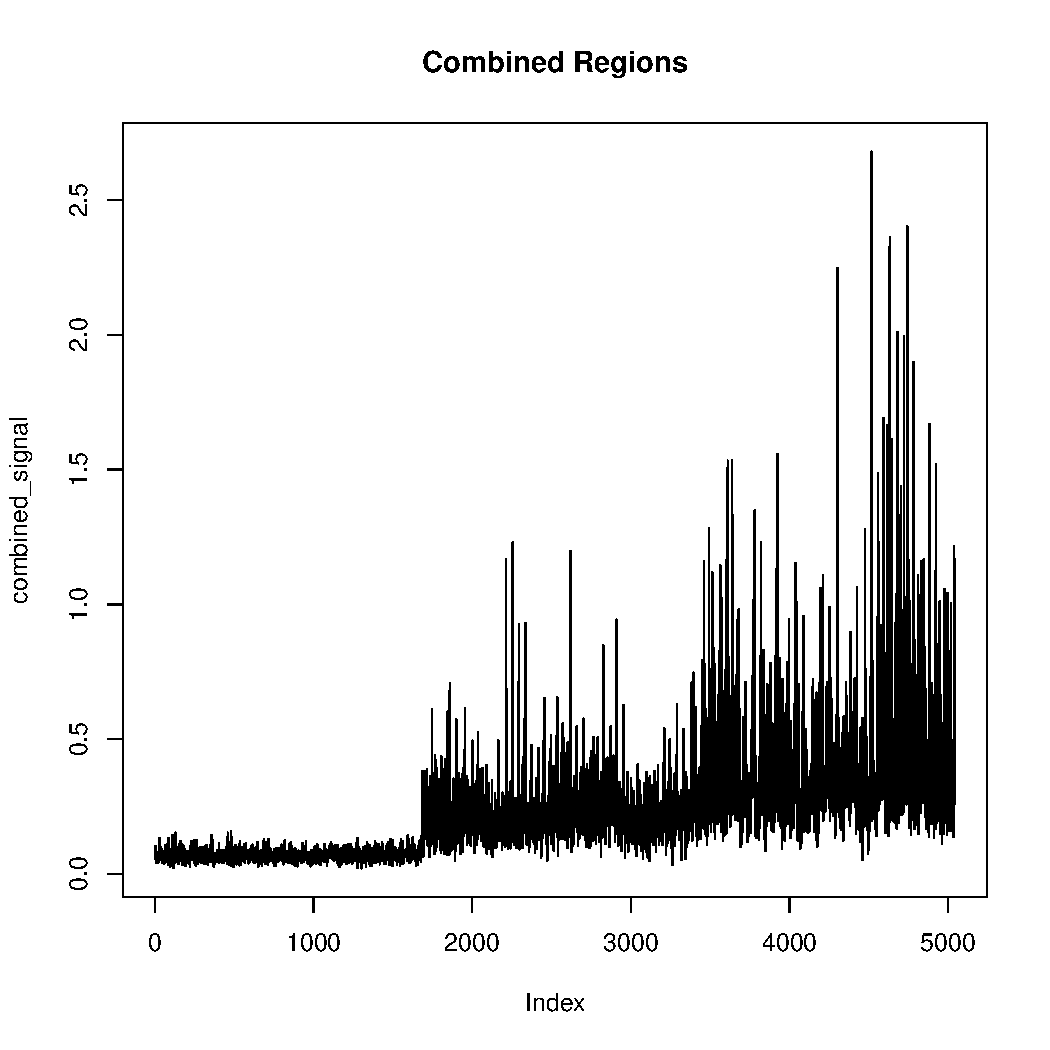
\includegraphics[width = \textwidth]{img/combined_regions.pdf}
	\caption{The three signals plotted next to each other as the "observed signal" }
	\label{fig:observededsignalfig}
\end{figure}

\noindent As one can observe in Figure \ref{fig:observededsignalfig}, the three areas \code{A}, \code{B}
and \code{C} are all quite distinct, where \code{A} have little activity and low average, while
\code{B} and \code{C} have more activity and higher average. meanwhile, \code{C} have more activity than
\code{B}, which is understandable, considering a city square would contain more activity than a ground square.

\subsection{Dummy covariates}
\label{ssec:dummycoviariates}
% TODO:
% Create two dummy covariates;
% Check the relationship between the mean of y and the dummy covariates;
\begin{figure}[!ht]
    \begin{subfigure}{.45\textwidth}
        \centering
        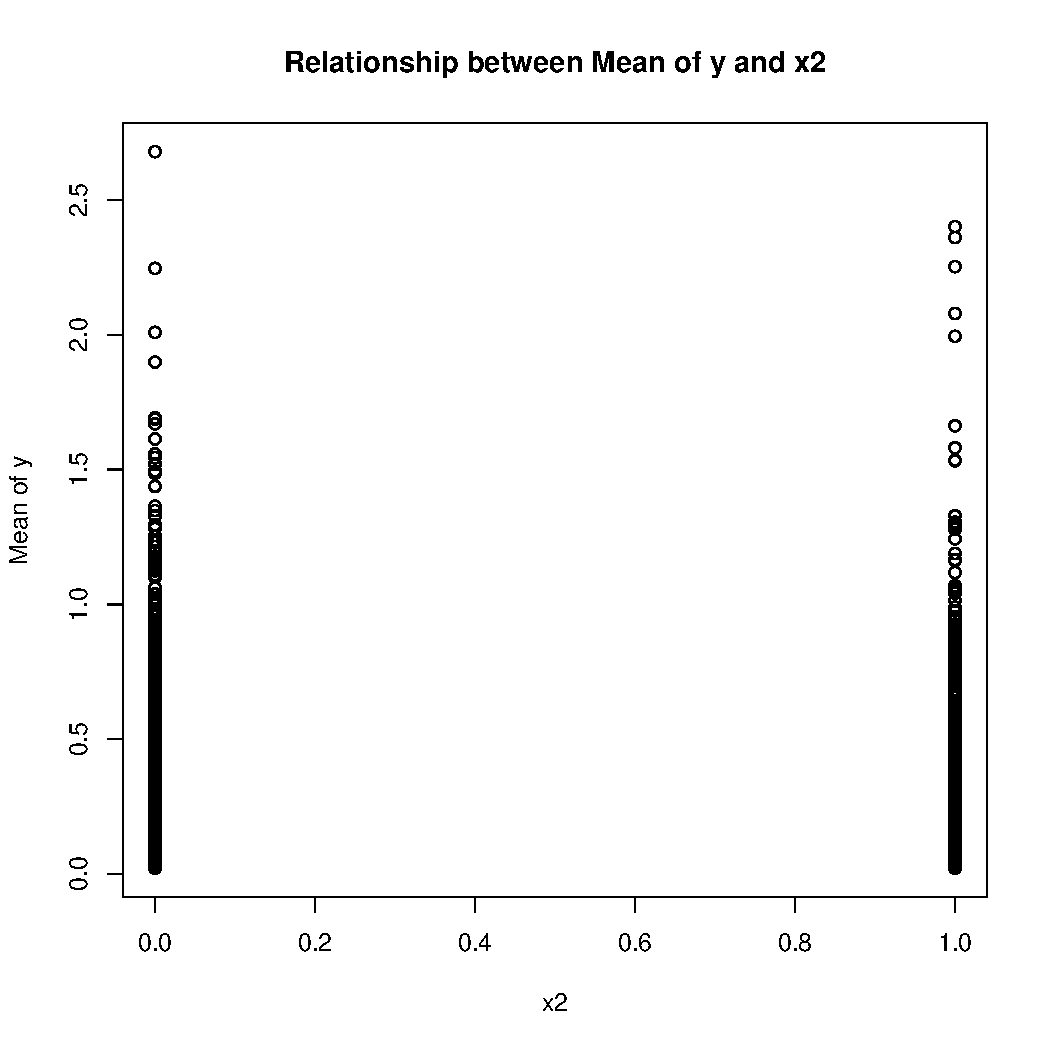
\includegraphics[width=\linewidth]{img/relationship_os_x2.pdf}
        \caption{Relationship between $y$ and $x2$}
        \label{fig:y_x2_rel}
    \end{subfigure}
    \begin{subfigure}{.45\textwidth}
        \centering
        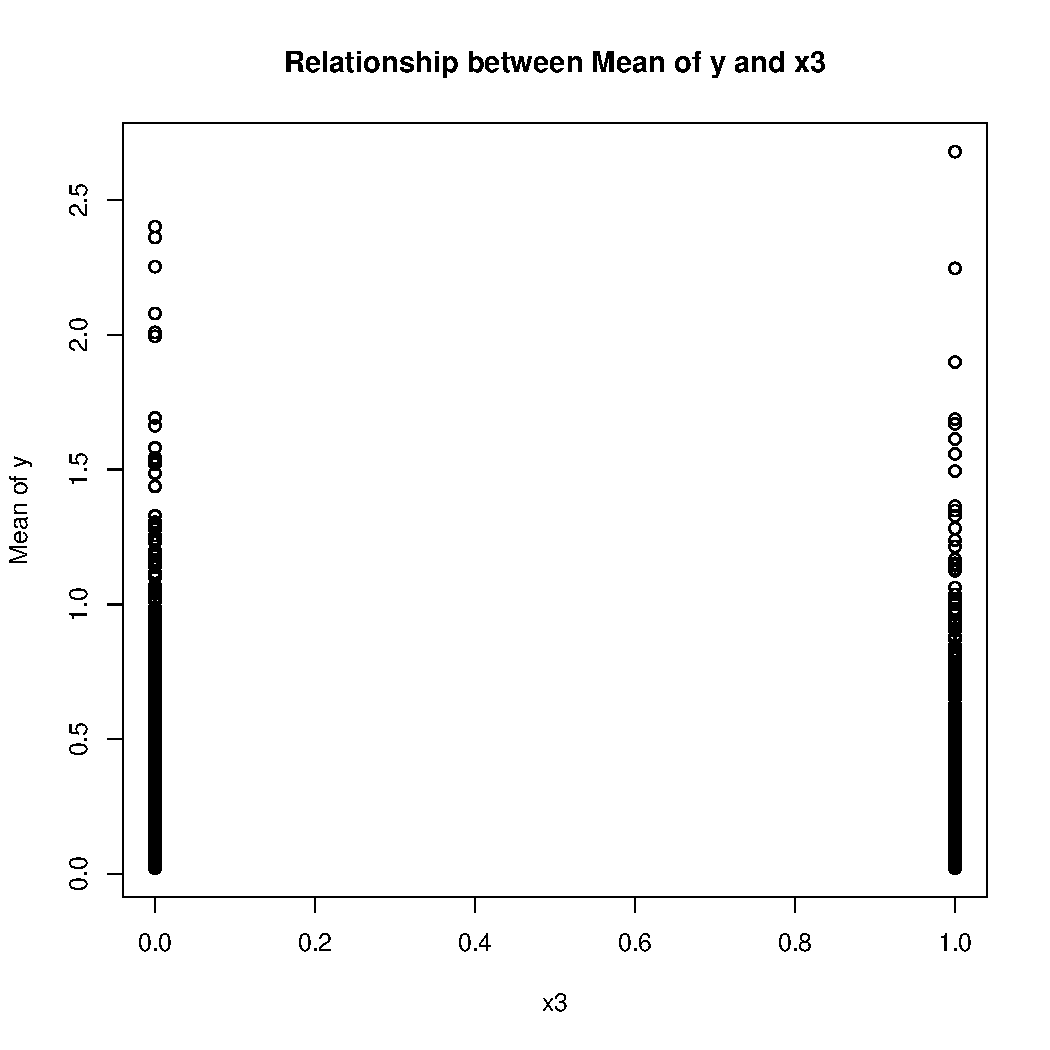
\includegraphics[width=\linewidth]{img/relationship_os_x3.pdf}
        \caption{Relationship between $y$ and $x3$}
        \label{fig:y_x3_rel}
    \end{subfigure}
    \caption{A plot of the relationship between the observed signal ($y$), and $x2$ and $x3$}
    \label{fig:ydummycovariatesfig}
\end{figure}

As is shown in the 

\subsection{Modeling}
\label{ssec:modeling}
% TODO:
% Fit the selected regression models. You can use the functions available on Canvas.
% Perform the detection theory. Are the covariates significant to the model? Are they introducing information about variations in y?
% Test the residuals. Is the model correctly specified? (Consider a residual vs index plot and check evidence of normality with a histogram, for example).
% Verify the determination coefficient for the fitted models;

\subsubsection{Gamma distribution}
\label{sssec:gamma}
\begin{figure}[!ht]
    \begin{subfigure}{.45\textwidth}
        \centering
        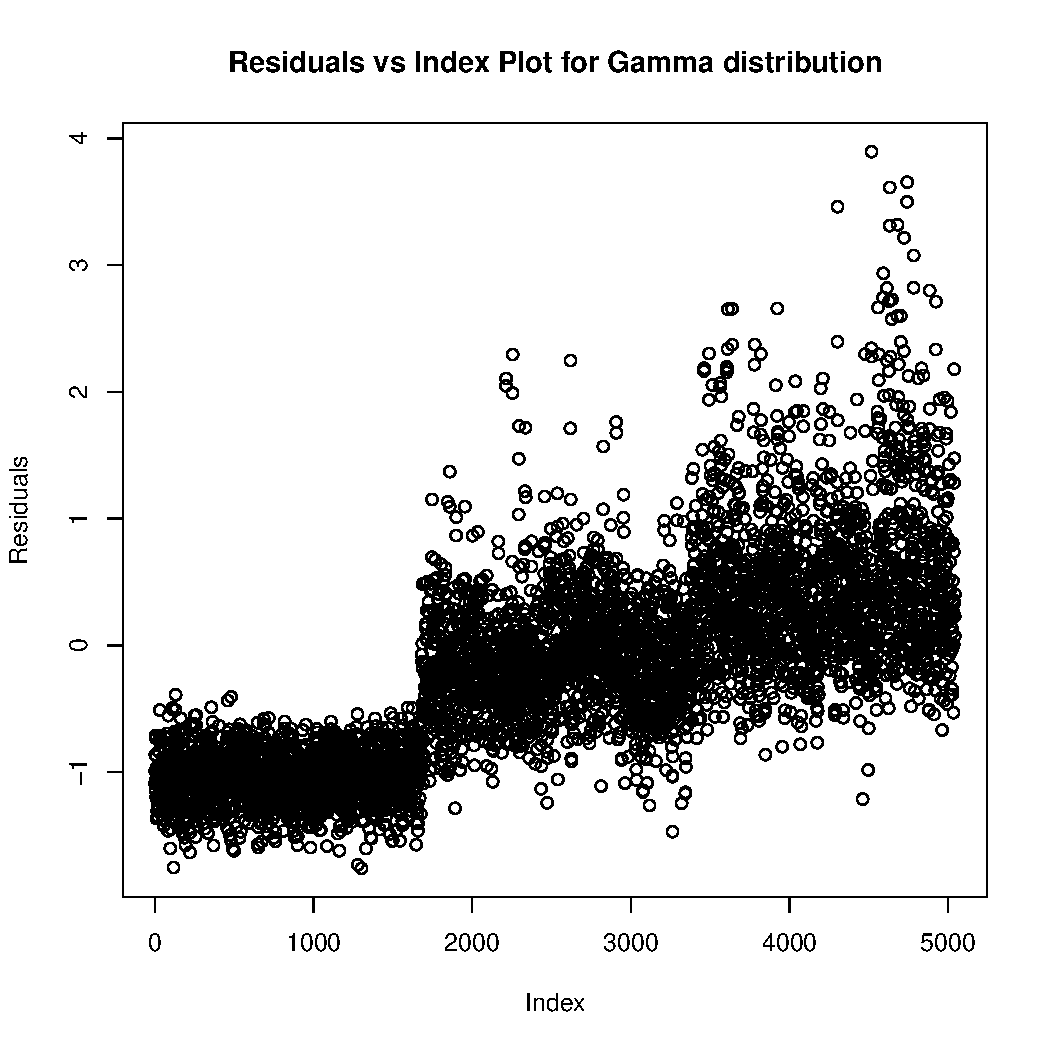
\includegraphics[width=\linewidth]{img/gamma_residuals.pdf}
        \caption{Scatter plot of the residuals}
        \label{fig:gammascatter}
    \end{subfigure}
    \begin{subfigure}{.45\textwidth}
        \centering
        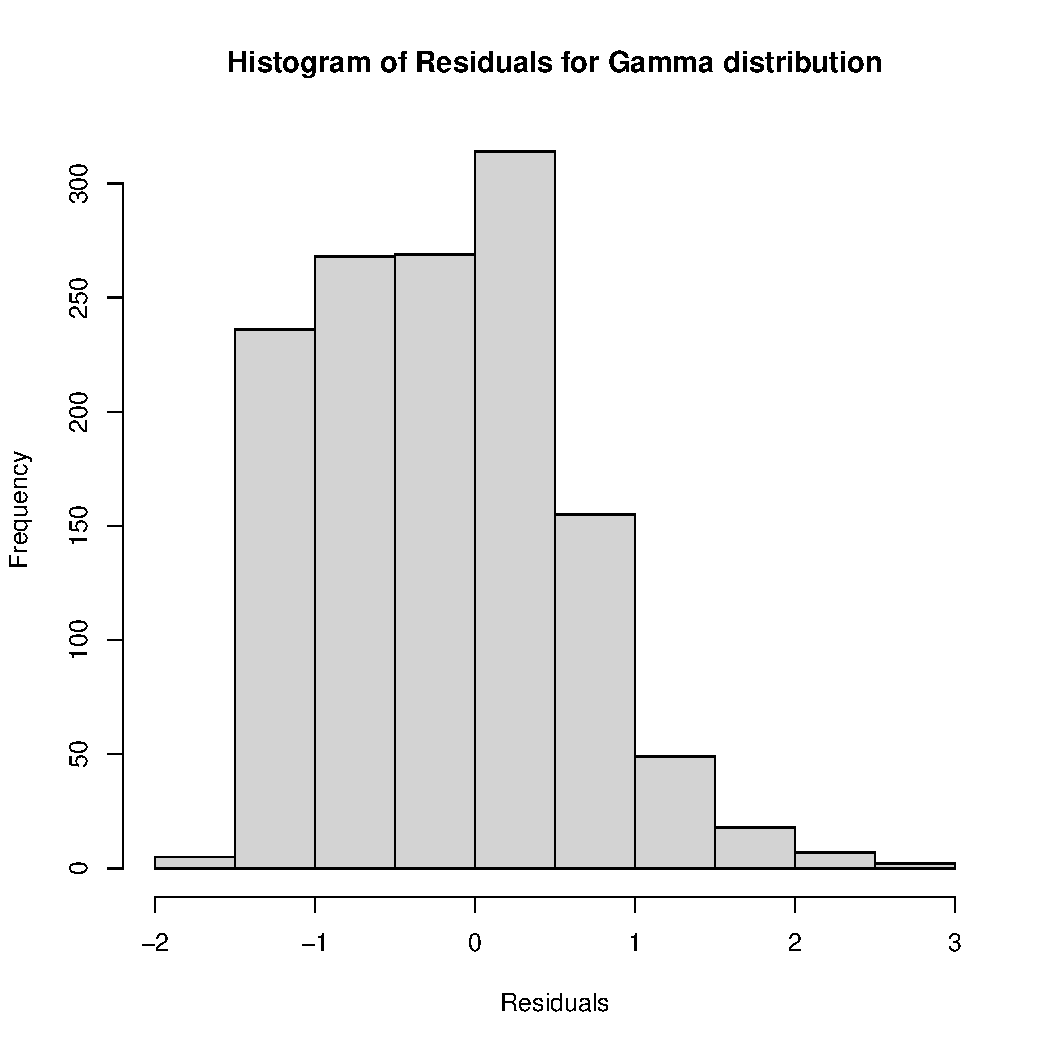
\includegraphics[width=\linewidth]{img/gamma_residuals_hist.pdf}
        \caption{Histogram plot of the distribution of residuals}
        \label{fig:gammahist}
    \end{subfigure}
    \caption{A graphic representation of the residuals of the GLM model with Gamma distribution}
    \label{fig:gammafig}
\end{figure}

\begin{longtable}{l|p{0.3\textwidth}|p{0.2\textwidth}}
	\textbf{Model} & \multicolumn{2}{r}{GLM with Gamma distribution} \\
	\hline
	\endhead
	\hline
	\multicolumn{3}{r}{\emph{Continued on the next page}}    \\
	\endfoot
	\hline
	\endlastfoot
	\hline
	 &  &  \\
	 \caption{GLM model with Gamma distribution}
	 \label{tab:part1res}
\end{longtable}

\subsubsection{Reyleigh distribution, devianvce residuals}
\label{sssec:reyleighdeviance}
\begin{figure}[!ht]
    \begin{subfigure}{.45\textwidth}
        \centering
        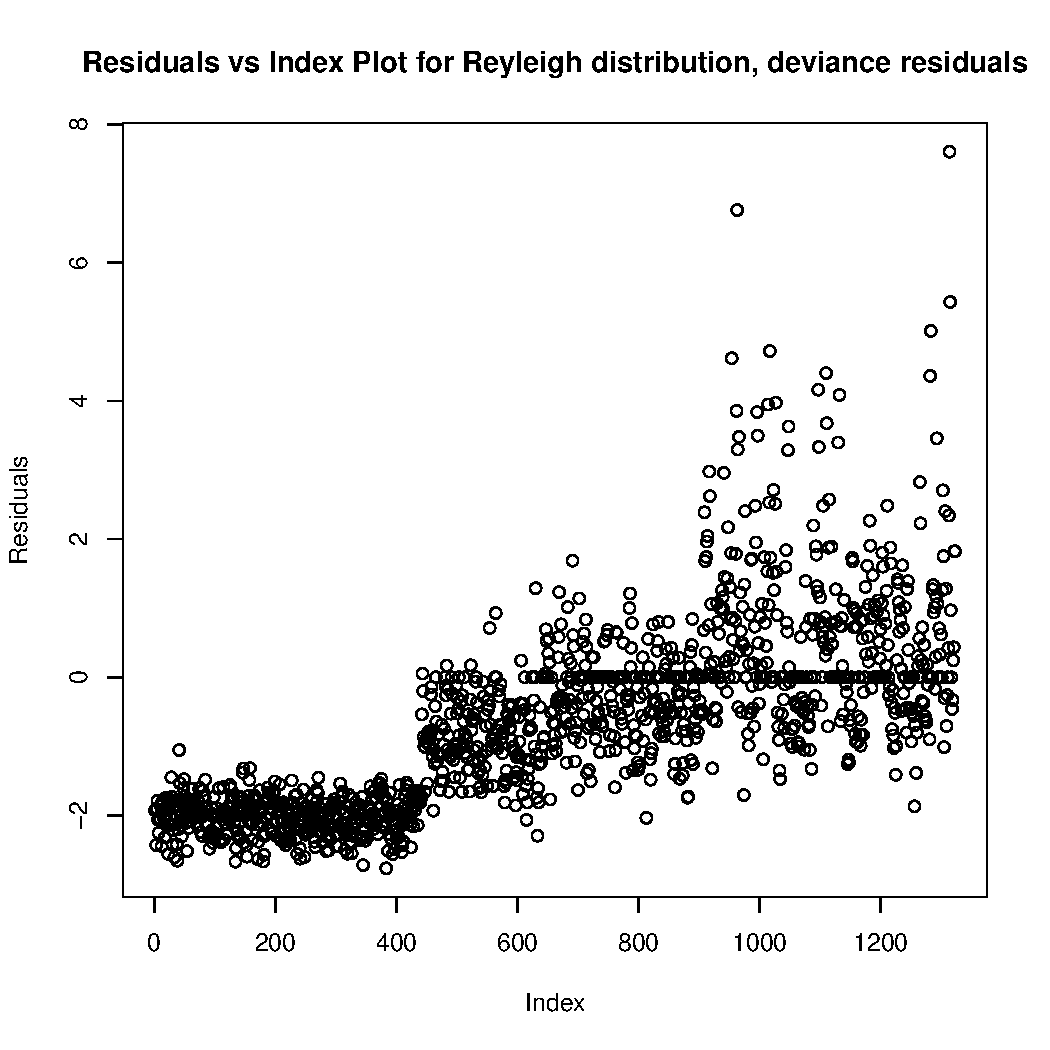
\includegraphics[width=\linewidth]{img/reyleigh_residuals_deviance.pdf}
        \caption{Scatter plot of the residuals}
        \label{fig:reyleighdeviancescatter}
    \end{subfigure}
    \begin{subfigure}{.45\textwidth}
        \centering
        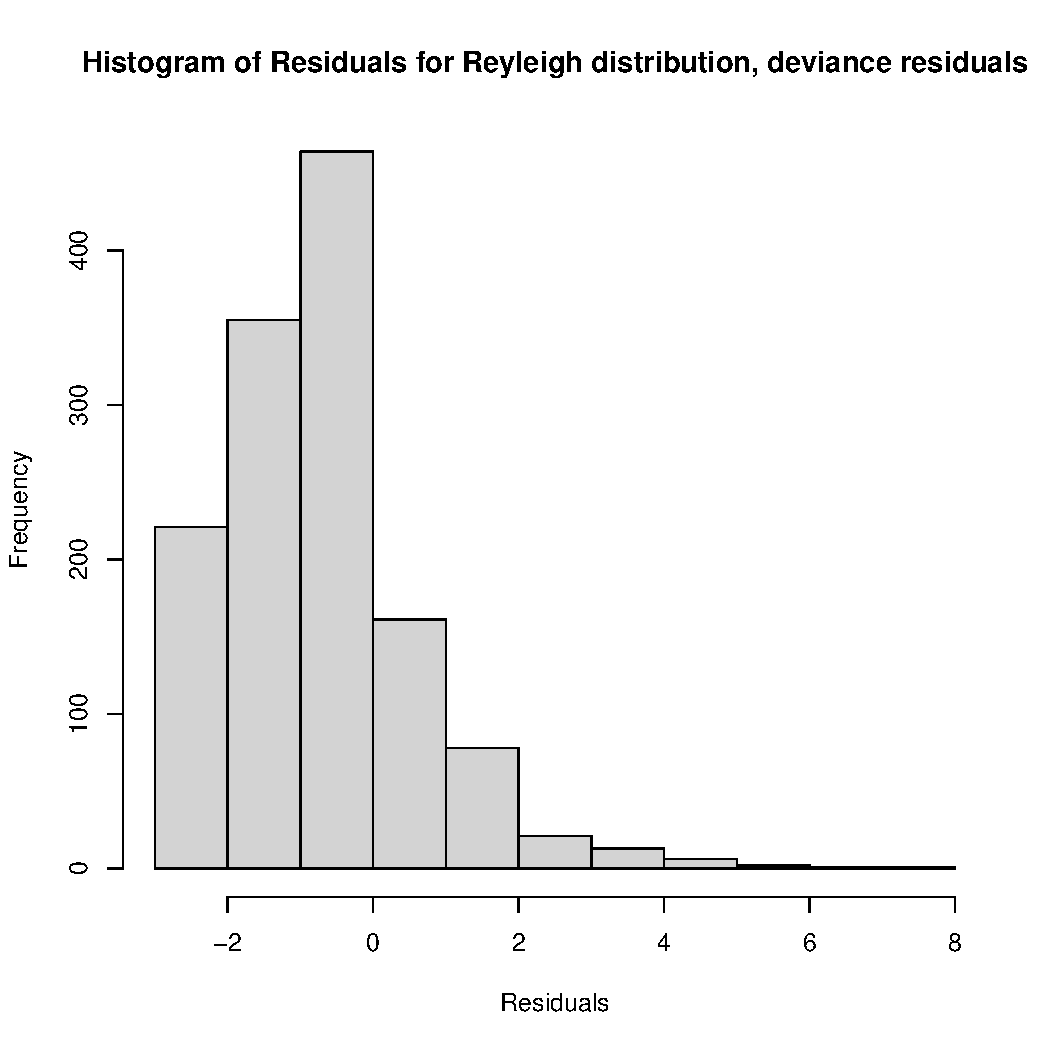
\includegraphics[width=\linewidth]{img/reyleigh_residuals_deviance_hist.pdf}
        \caption{Histogram plot of the distribution of residuals}
        \label{fig:reyleighdeviancehist}
    \end{subfigure}
    \caption{A graphic representation of the deviance residuals of the model with Reyleigh distributions}
    \label{fig:reyleighdeviancefig}
\end{figure}

\begin{longtable}{l|p{0.3\textwidth}|p{0.2\textwidth}}
	\textbf{Model} & \multicolumn{2}{r}{Deviance residuals for model with Reyleigh distribution} \\
	\hline
	\endhead
	\hline
	\multicolumn{3}{r}{\emph{Continued on the next page}}    \\
	\endfoot
	\hline
	\endlastfoot
	\hline
	 &  &  \\
	 \caption{Deviance residuals for model with Reyleigh distribution}
	 \label{tab:reyleighdeviancetab}
\end{longtable}

\subsubsection{Reyleigh distribution, with quantile residuals}
\label{sssec:reyleighquantile}
\begin{figure}[!ht]
    \begin{subfigure}{.45\textwidth}
        \centering
        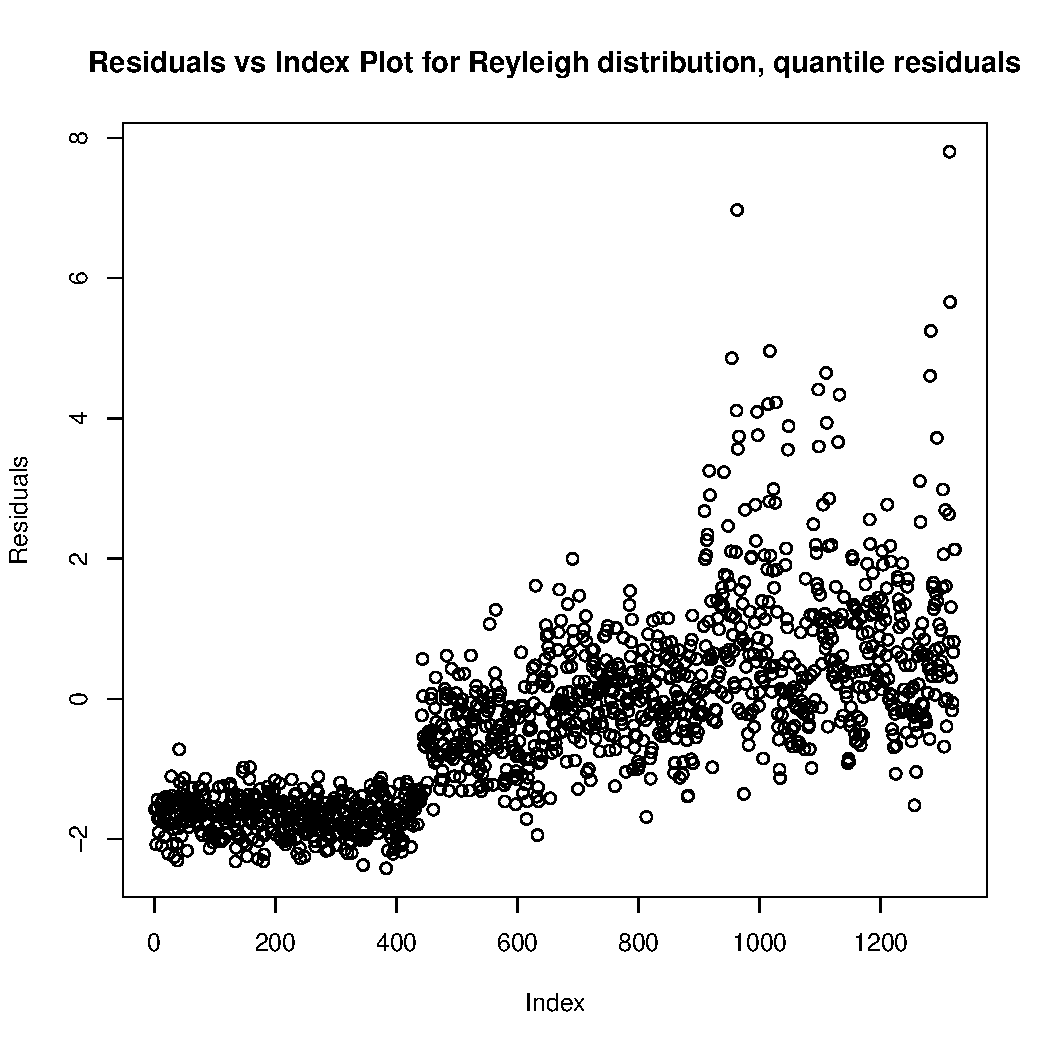
\includegraphics[width=\linewidth]{img/reyleigh_residuals_quantile.pdf}
        \caption{Scatter plot of the residuals}
        \label{fig:reyleighquantilescatter}
    \end{subfigure}
    \begin{subfigure}{.45\textwidth}
        \centering
        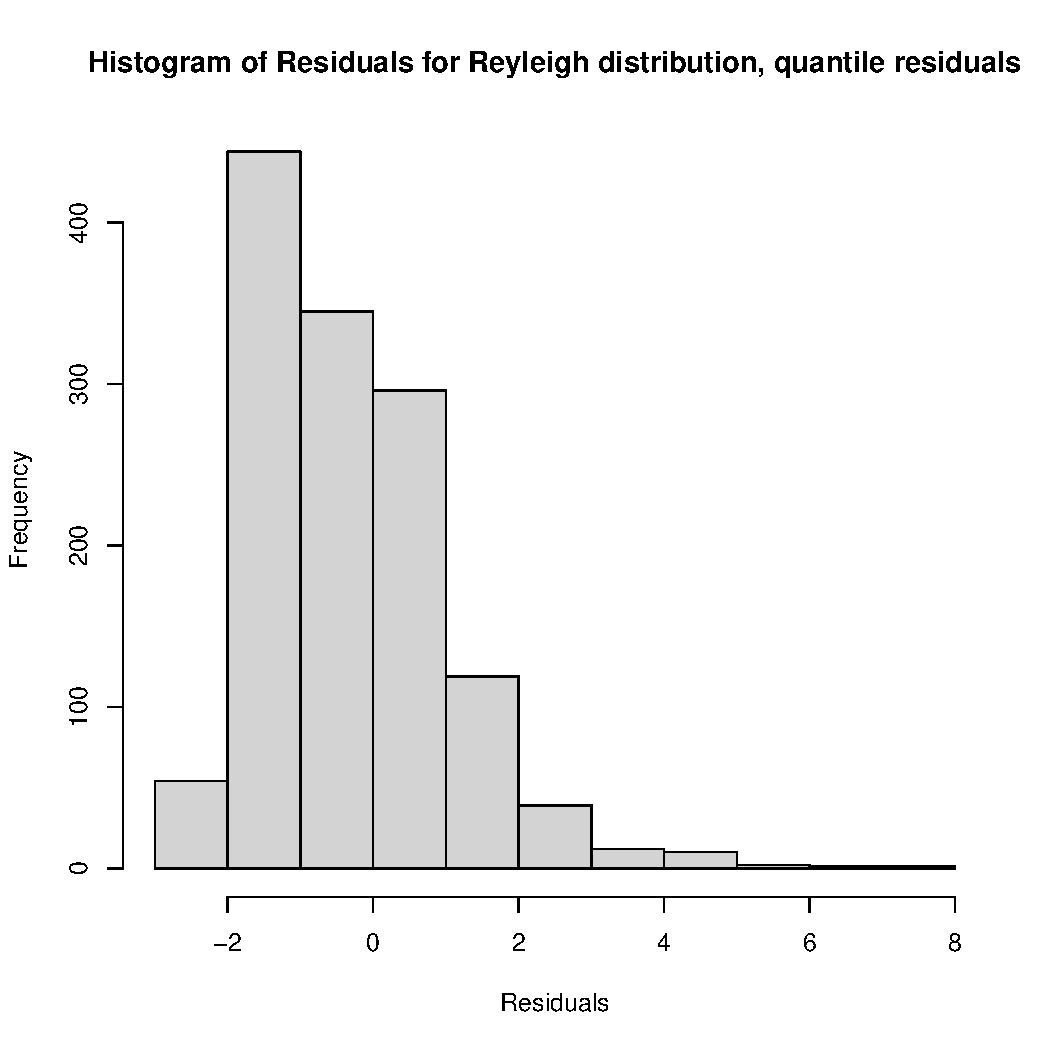
\includegraphics[width=\linewidth]{img/reyleigh_residuals_quantile_hist.pdf}
        \caption{Histogram plot of the distribution of residuals}
        \label{fig:reyleighquantilehist}
    \end{subfigure}
    \caption{A graphic representation of the quantile residuals of the model with Reyleigh distribution}
    \label{fig:reyleighquantilefig}
\end{figure}

\begin{longtable}{l|p{0.3\textwidth}|p{0.2\textwidth}}
	\textbf{Model} & \multicolumn{2}{r}{Quantile residuals for model with Reyleigh distribution} \\
	\hline
	\endhead
	\hline
	\multicolumn{3}{r}{\emph{Continued on the next page}}    \\
	\endfoot
	\hline
	\endlastfoot
	\hline
	 &  &  \\
	 \caption{Quantile residuals for model with Reyleigh distribution}
	 \label{tab:reyleighquantiletab}
\end{longtable}

\subsubsection{Reyleigh distribution, with standardized residuals}
\label{sssec:reyleighstandardized}
\begin{figure}[!ht]
    \begin{subfigure}{.45\textwidth}
        \centering
        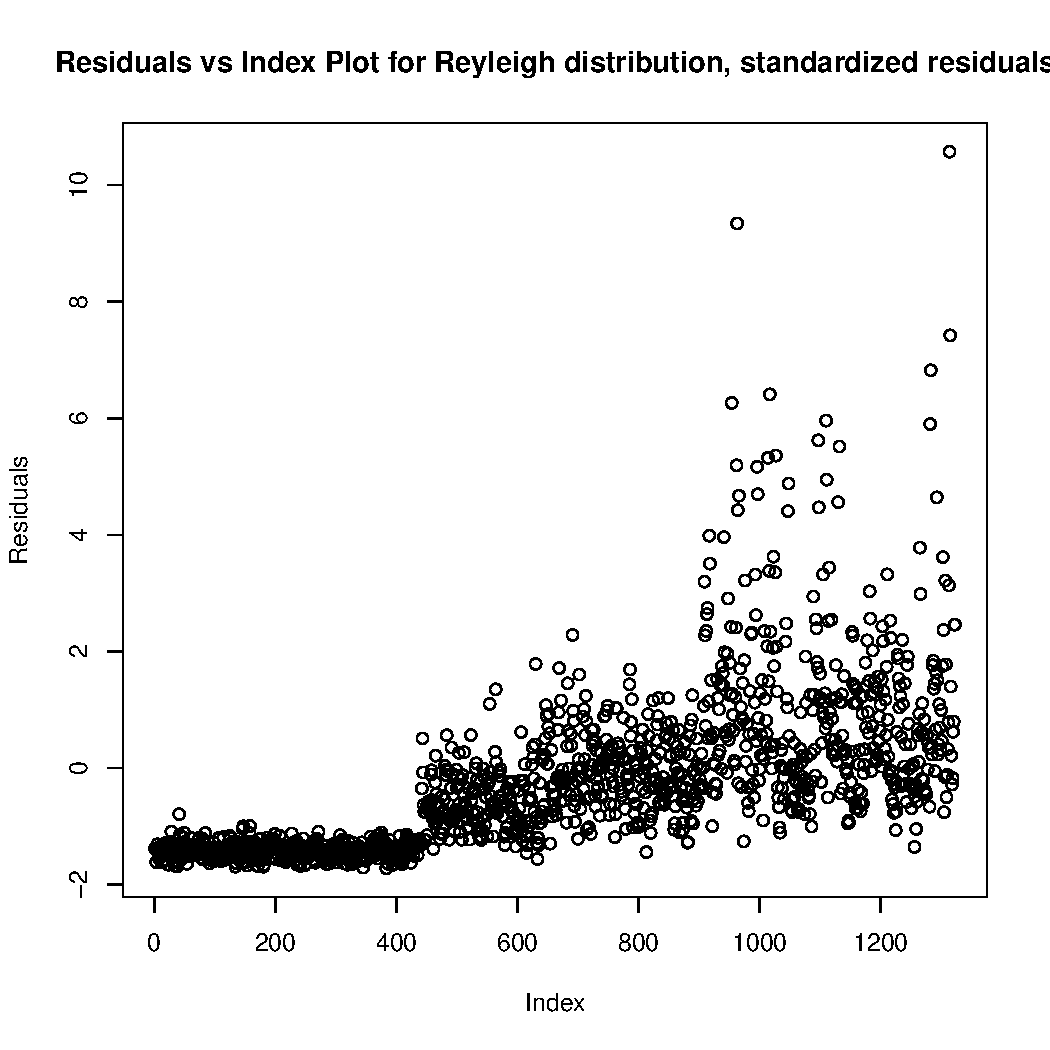
\includegraphics[width=\linewidth]{img/reyleigh_residuals_standardized.pdf}
        \caption{Scatter plot of the residuals}
        \label{fig:reyleighstandardizedscatter}
    \end{subfigure}
    \begin{subfigure}{.45\textwidth}
        \centering
        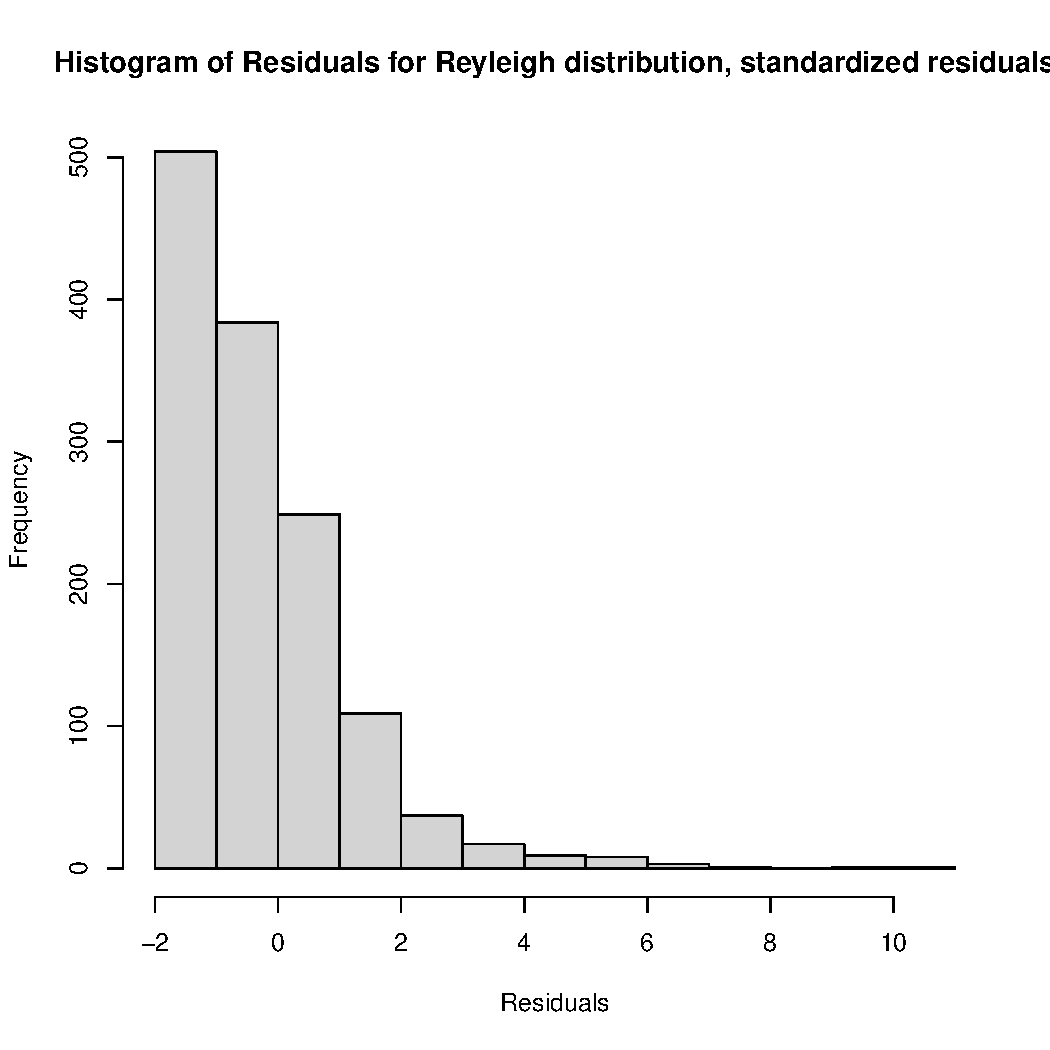
\includegraphics[width=\linewidth]{img/reyleigh_residuals_standardized_hist.pdf}
        \caption{Histogram plot of the distribution of residuals}
        \label{fig:reyleighstandardizedhist}
    \end{subfigure}
    \caption{A graphic representation of the standardized residuals of the model with Reyleigh distribution}
    \label{fig:reyleighstandardizedfig}
\end{figure}

\begin{longtable}{l|p{0.3\textwidth}|p{0.2\textwidth}}
	\textbf{Model} & \multicolumn{2}{r}{Standardized residuals for model with Reyleigh distribution} \\
	\hline
	\endhead
	\hline
	\multicolumn{3}{r}{\emph{Continued on the next page}}    \\
	\endfoot
	\hline
	\endlastfoot
	\hline
	 &  &  \\
	 \caption{Standardized residuals for Reyleigh distribution}
	 \label{tab:reyleighstandardizedtab}
\end{longtable}

\subsubsection{Normal distribution}
\label{sssec:gaussian}
\begin{figure}[!ht]
    \begin{subfigure}{.45\textwidth}
        \centering
        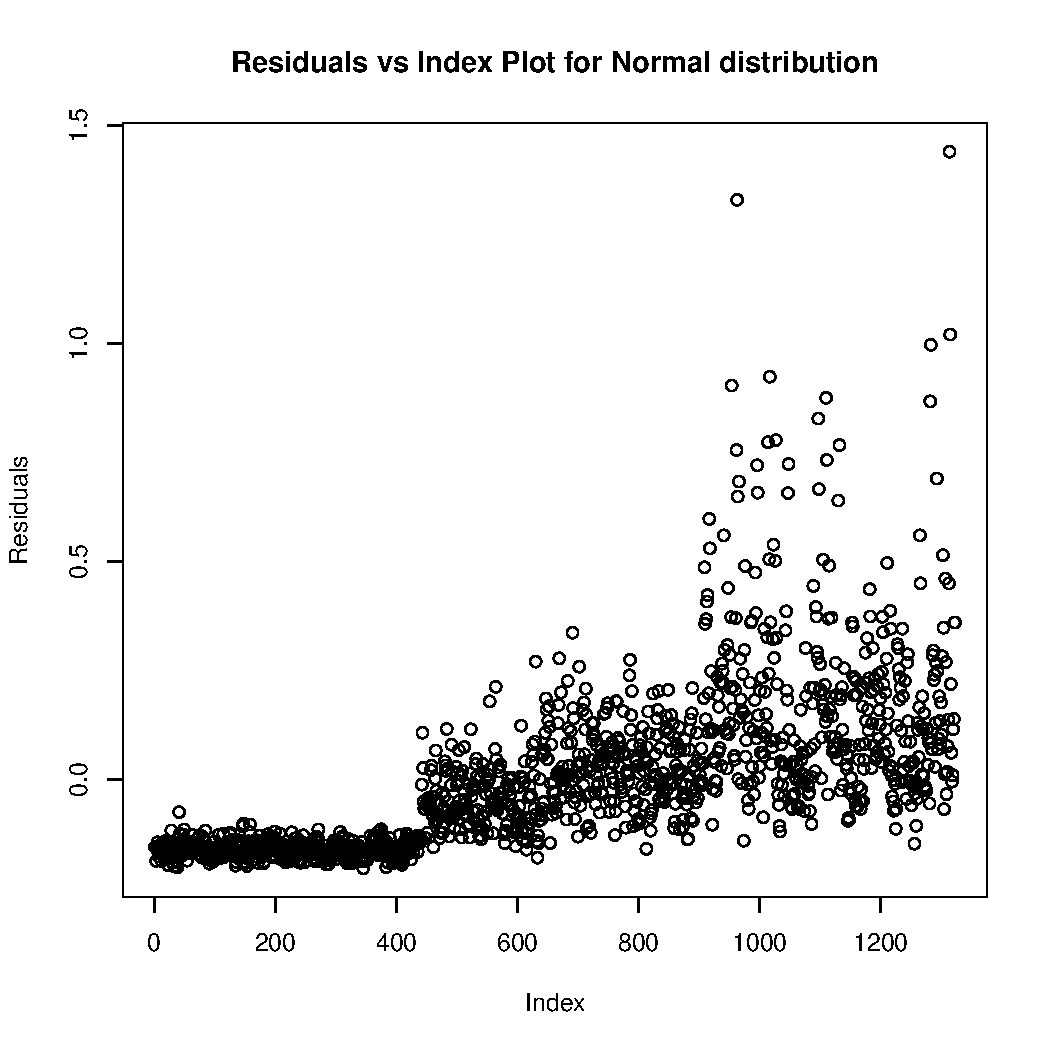
\includegraphics[width=\linewidth]{img/normal_residuals.pdf}
        \caption{Scatter plot of the residuals}
        \label{fig:gaussianscatter}
    \end{subfigure}
    \begin{subfigure}{.45\textwidth}
        \centering
        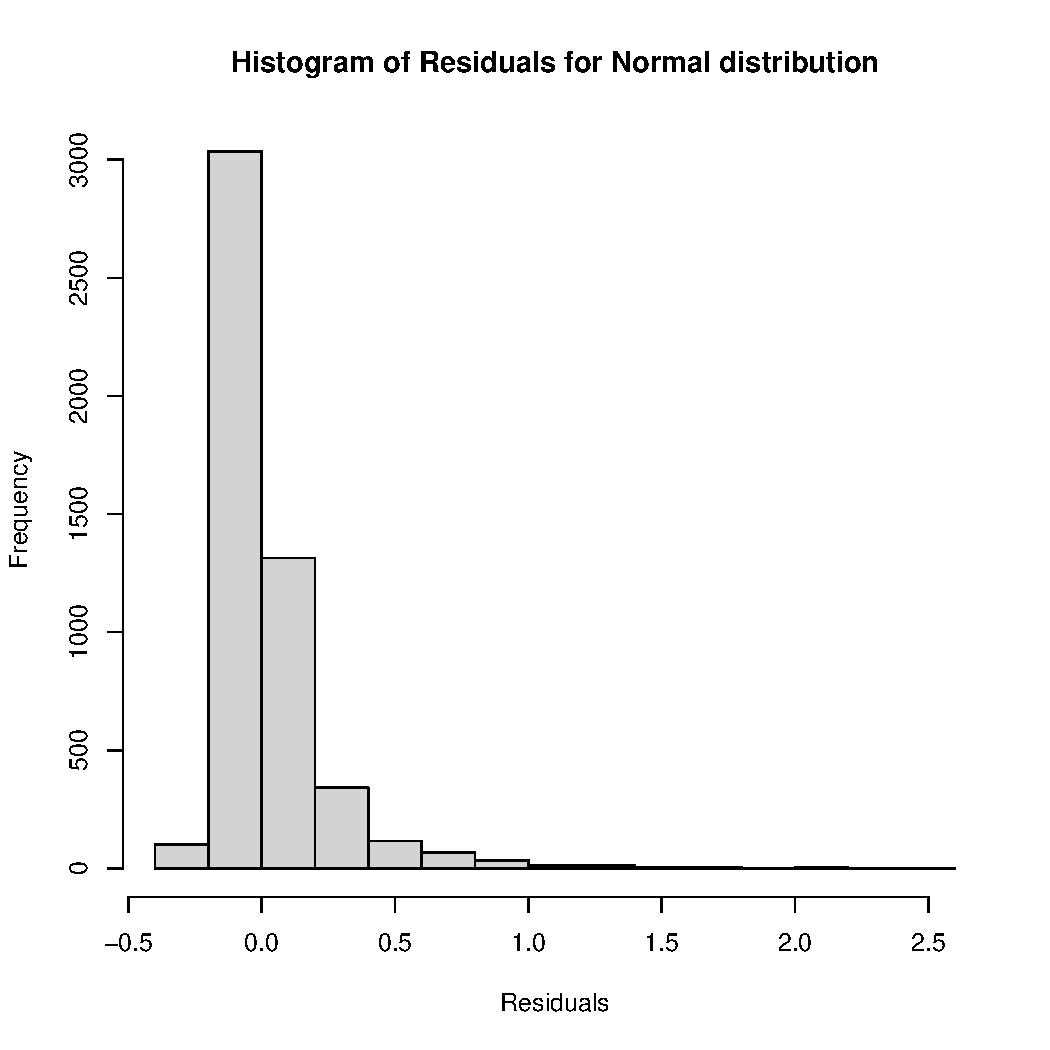
\includegraphics[width=\linewidth]{img/normal_residuals_hist.pdf}
        \caption{Histogram plot of the distribution of residuals}
        \label{fig:gaussianhist}
    \end{subfigure}
    \caption{A graphic representation of the residuals of the GLM model with Normal (Gaussian) distribution}
    \label{fig:gaussianfig}
\end{figure}

\begin{longtable}{l|p{0.3\textwidth}|p{0.2\textwidth}}
	\textbf{Model} & \multicolumn{2}{r}{GLM with Normal distribution} \\
	\hline
	\endhead
	\hline
	\multicolumn{3}{r}{\emph{Continued on the next page}}    \\
	\endfoot
	\hline
	\endlastfoot
	\hline
	 &  &  \\
	 \caption{Normal distribution}
	 \label{tab:gaussiantab}
\end{longtable}

\subsection{Conclusion}
\label{ssec:conclusion}
% TODO:
% What is the most accurate model for such data, considering detection and modeling evaluation?

\newpage
\section{Part 2}
\subsection{Results}
\begin{longtable}{l|p{0.3\textwidth}|p{0.2\textwidth}}
	\textbf{Layer} & \textbf{Output shape} & \textbf{Params} \\
	\hline
	\endhead
	\hline
	\multicolumn{3}{r}{\emph{Continued on the next page}}    \\
	\endfoot
	\hline
	\endlastfoot
	\hline
	 &  &  \\
	\caption{Part 2 result table}
	\label{tab:part2res}
\end{longtable}
\subsection{Analysis}

\end{document}